\chapter{مفاهیم}
\part*{جلسهٔ اول}
\section{کارساز وب چیست؟}
\let\oldabstract\abstract
کارساز وب سیستم یا سامّانه‌ای است که  در هنگام درخواست کاربر برای دریافت اطلاعات و داده‌های مورد نظر، به وی پاسخ داده و به ارائه خدمات می‌پردازد. کارساز وب را با نام خدمات‌دهنده یا خدمتگزار نیز می‌شناسند. کارساز وب معمولا از یک سیستم‌عامل به همراه برخی ابزارهای مورد نیاز برای پاسخگویی در خور نیاز مشتریان خود است که اگر درخواستی دریافت کرد بتواند به آن پاسخ مناسبی دهد. مثلا برای ارائه خدمات به صورت ابر‌متن و اچ‌تی‌تی‌پی، باید یک نرم‌افزار کارساز وب مانند آی‌آی‌اس یا آپاچی بهره‌مند باشد. علاوه بر آن برای توسعه برنامه‌ها نیاز به برخی کتابخانه‌ها و زبان‌های برنامه‌نویسی دارد تا بتواند کد‌های نوشته شده را تفسیر کند.

اصلی‌ترین استفاده از یک کارساز وب همان استفاده برای انتقال مطالب در قالب اچ‌تی‌ام‌ال است که یا به صورت مستقیم داده‌ها اچ‌تی‌امل هستند یا به صورت کد‌های پویا نوشته شده‌اند و به زبان اچ‌تی‌ام‌ال تفسیر خواهند شد. علاوه بر این یک کارساز وب قادر است به ارائه محتوای چندرسانه‌ای در بستر اچ‌تی‌ام‌ال یا دیگر پروتکلها بپردازد که این مهم با استفاده از اچ‌تی‌ام‌ال ویرایش پنجم  یا فلش قابل انجام است. 

ویژگی‌های یک کارساز وب که تقریبا در تمامی موارد این چنین بوده و از ویژگی‌های یکسانی برخوردارند، شامل موارد زیر است.
\begin{itemize}
\item
	شناسایی: درخواست شناسایی اختیاری قبل از اجازه دسترسی به انواع منابع
\item
	پشتیبانی از اطلاعات به صورت ایستا و ثابت مانند فایل‌های متنی و یا اچ‌تی‌ام‌ال ساده و همچنین اطلاعات پیچیده و پویا  مانند تفسیر کدها و اسکریپت‌های نوشته شده تحت زبان‌های اسکریپتی و مبنی‌بر وبی چون پی‌اچ‌پی، پرل، ای‌اس‌پی و حتی پایتون.
\item
	پشتیبانی از اچ‌تی‌تی‌پی‌اس برای اجرای امن و مطمئن به وسیله درگاه  ۴۴۳ به جای ۸۰، که معمولا برای چنین اتصالاتی رزرو شده است.
	قابلیت فشرده‌سازی مطالب با استفاده از روش‌های جی‌زیپ «GZIP» که باعث کاهش بار ترافیک کارساز وب می‌شود.
\item
	قابلیت پشتیبانی از بزرگ‌فایل‌ها و یا بزرگ‌داده‌ها به شکلی که در هنگام پردازش و نگاهداری چنین اطلاعاتی دچار مشکل نشده و سیستم دچار تاخیر و یا توقف ناگهانی نشود.
\item
	کنترل کردن پهنای باند: تا سرعت پاسخها را محدود کند و شبکه را به دلیل به وجود آمدن اختلالات یا به دلیل عدم پاسخگویی دچار مشکل نکند و قادر باشد به تمامی موارد درخواستی پاسخ مناسبی ارائه دهد. برخی مواقع به دلیل هجوم انبوهی از مراجعه‌کنندگان و درخواست‌های مختلف ممکن است سرور دچار سکته‌ای کوتاه و یا بلند در ارائه خدمات شود که در برخی موارد منجر به توقف و کاهش کیفیت ارائه خدمات کامل خواهد شد که اگر یک کارساز وب بهتر، ترافیک داده‌ها را مدیریت کند، کارساز وب کمتر دچار مشکل خواهد شد.
	
\end{itemize}
\section{مدیر پایگاه‌ داده مای‌اس‌کیو‌ال و زبان برنامه‌نویسی پی‌اچ‌پی}
\label{2}
\index{مدیر پایگاه‌ داده مای‌اس‌کیو‌ال و زبان برنامه‌نویسی پی‌اچ‌پی}
 
استفاده از بانک‌های اطلاعاتی برای نگاهداری اطلاعات، قابلیتی است که در اکثر پایگاه‌های اینترنتی مورد استفاده قرار می‌گیرد. پایگاه‌ها‌داده و یا بانک‌های اطلاعاتی اطلاعات را در جدولهایی مشخصی و در فیلدهای مشخص ذخیره می‌کنند که برای دسترسی به اطلاعات هر فیلد می‌توان از شاخص نام فیلد و اندیس داده استفاده کرد. به عنوان مثال برای دستیابی به اطلاعات علی ربیعی که در سطر ۸۰ و با اندیس و شاخص کلیدی ۸۰ ذخیره شده‌است می‌توان با مشخصه فیلد و شاخص کلیدی آن، به نام فرد بیان شده دسترسی یافت. به طور کلی به مجموعه‌ای از داده‌ها و اطلاعات که به صورت طبقه‌بندی شده و منظم و بر اساس ساختار خاصی گرد هم آمده‌اند را یک پایگاه داده می‌خوانند. پایگاه داده‌ها برای حمایت از عملیات داخلی سازمان‌ها و زیر بنای تعامل برخط  با مشتریان و توسعه‌دهندگان. استفاده می‌شود. نمونه‌هایی از برنامه‌های کاربردی پایگاه داده شامل سیستم کتابخانه کامپیوتری، سیستم رزرو پرواز و .. هستند.

برای مدیریت این پایگاه‌های داده ا دی‌بی‌ام‌اس‌ها «DBMS» استفاده می‌شود که به معنای سیستم مدیریت پایگاه داده است. این سیستم‌ها برای ارائه ابزار و قابلیت‌های مختلف برای دسترسی و تغییر در این پایگاه‌های داده طراحی گشته‌اند. به طور کلی دی‌بی‌ام‌اس یک سیستم نرم‌افزار پیچیده تکامل یافته است. از دی‌بی‌ام‌اس‌های مطرح می‌توان به ماریا‌دی‌بی، مای‌اس‌کیو‌ال، اس‌کی‌یو‌ال سرور و اوراکل اشاره کرد. مای‌اس‌کیو‌ال یک دی‌بی‌ام‌اس متن‌باز است که از دو نسخه رایگان و پولی با پشتیبانی تجاری برخوردار است. با این حال بعد از خریده شدن شرکت سان توسط اوراکل، ابزار جدید با نام ماریا‌دی‌بی از آن منشعب شد که از ویژگی‌های مای‌اس‌کیو‌ال برخوردار است. معمولا در توزیع‌های گنو/لینوکس از یکی از این دو ابزار استفاده می‌شود. در توزیع اوبونتو از مای‌اس‌کیو‌ال شرکت اوراکل استفاده می‌شود.

\begin{figure}

\includegraphics[width=.9\textwidth ,height=.50\textwidth]{Pic/InformationHidingHierarch}
\caption{ نمادهای LAMP}
\label{LampLogo}
\end{figure}

\section{دلیل انتخاب گنو/لینوکس و توزیع اوبونتو}
\subsection{نگاهی مختصر بر تاریخچه گنو/لینوکس}
\label{SteganalysisIntro}

در ابتدا نگاهی به تاریخچه این سیستم‌عامل خواهیم انداخت، لینوکس در سال ۱۹۹۲ تحت مجوز گنو/جی‌پی‌ال اجازه انتشار یافت و دو سال بعد لینوکس ویرایش ۱٫۰ منتشر شد. در سال ۱۹۹۴ شرکت ردهت به وسیله باب یانگ 
\lr{(Bob Young)}
 و مارک اوینگ 
 \lr{(Marc Ewing)}
  تاسیس شد و یک سال بعد گنو/لینوکس و سایر نرم‌افزارهای آزاد به همراه هسته آماده شده‌ای با نام لینوکس، به طور گسترده‌ای در اینترنت انتشار یافتند. این سیستم‌عامل که امروز بیش از ۱۰۰ میلیون کاربر دارد از خانواده یونیکس (شبه یونیکس) به شمار می‌رود و از کلیه ویژگی‌های آن بهره می‌برد. سال‌ها قبل با وجود افزایش تولیدات سخت افزاری، مشکل بزرگی بر سر راه کاربران رایانه وجود داشت و آن وجود نداشتن سیستم‌های عامل مختلف، برای انتخاب و استفاده بود. رایانه‌های ساخته شده به وسیله شرکت اپل با سیستم عامل انحصاری خود گزینه مناسبی بودند، امّا قیمت بالا، آنها را از دسترس بیشتر افراد دور می ساخت. یونیکس، دیگر انتخاب موجود، با کد اصلی محافظت شده آن قدر گران قیمت بود که جز چند دانشگاه و آزمایشگاه، دیگران امکان استفاده از آن را نداشتند.
\subsection{ویژگی های سیستم عامل گنو/لینوکس}
امروزه سیستم‌عامل گنو/لینوکس در ابر رایانه‌ها و ایستگاه‌های کاری، رایانه‌های رومیزی و سیستم‌های اتوماسیون اداری به کار گرفته می‌شود. همچنین ریز پردازنده‌های مورد استفاده در تجهیزات پزشکی و نظامی و حتی تلفن‌های همراه نیز آن را به کار می‌گیرند. از آن جا که گنو/لینوکس نسبت به ویندوز از امنیت بیشتری برخوردار است، شرکت‌های با فعالیت محرمانه، برای ارائه سیستم‌های امنیتی ـ حفاظتی خود از این سیستم عامل بهره می‌گیرند. مهم‌ترین ویژگی‌های سیستم عامل گنو/لینوکس را می‌توان به صورت زیر بر شمرد.

۱)  پایین بودن هزینه‌ها: گنو/لینوکس یک سیستم‌عامل رایگان است و بیشتر توزیع‌های آن به راحتی از طریق سایت‌های اینترنتی (بصورت کاملا قانونی) قابل دریافت هستند. همواره هزاران صفحه اطلاعات رایگان برای نصب و نگهداری آن در اینترنت یا در ویکی‌ها موجود است. البته بعضی از توزیع‌های تجاری گنو/لینوکس نیز وجود دارند که قیمت آنها به مراتب پایین‌تر از ویندوز و دیگر سیستم‌عامل‌های تجاری موجود است.

۲) امنیت و پایداری: گنو/لینوکس، امنیت یونیکس را به همراه دارد. باز بودن کد اصلی گنو/لینوکس سبب شده است متخصصان با همکاری یکدیگر به رفع نقایض امنیتی آن بپردازند و یکی از امن‌ترین سیستم‌های عامل را به وجود آورند. این پایداری سبب شده است که تا سال 1994 میلادی حدود 30٪ از سرورهای دنیا، از خانواده این سیستم عامل استفاده کنند. نکته بسیار مهم این است که تاکنون هیچ گونه کرم و ویروسی، مشابه آن چه برای ویندوز مشاهده می‌کنیم، برای این نوع از سیستم های عامل نوشته نشده است، و اگر روزی این اتفاق افتاد بدلیل متن‌باز بودن، سریعا باگ مربوطه برطرف خواهد شد و از گسترش آن جلوگیری بعمل خواهد آمد.

۳)  تطبیق با آخرین سخت افزارها : از آنجا که این سیستم عامل در دنیا علاقه‌مندان زیادی دارد، به محض ساخته شدن قطعات سخت‌افزاری جدید، راه‌اندازهای آن‌ها نیز در اینترنت انتشار می‌یابد. به علاوه برخی از توزیع‌های گنو/لینوکس با حداقل امکانات سخت افزاری قابل اجرا هستند به طوری که می توانند از گرداننده دیسک نوری یا فلاپی دیسک! و حافظه‌های جانبی قابل حمل دیگر، به اجرا در آمده و به کار گرفته شوند.

۴) گنو/لینوکس دارای چند محیط گرافیکی و حالت متنی مشابه سیستم‌عامل داس است. تنوع این محیط‌ها سبب شده است استفاده کاربران از این سیستم عامل چند کاربره راحت‌تر و جذابتر شود. کی‌دی‌ای و گنوم دو عدد از معروف‌ترین محیط‌های گرافیکی این سیستم عامل هستند.

۵) قابلیت تطبیق با نیازها: وجود کد اصلی باز به برنامه‌نویسان آشنا به زبانهای اسمبلی، C و C++ یا حتی پرل, پایتون اجازه می‌دهد که سیستم عامل را مطابق نیاز شرکت و یا اداره و سازمان خود بسازند. البته برای این کار، برنامه نویس باید اصول طراحی سیستم عامل را بداند. این قابلیت سبب شده است که گنو/لینوکس در مقایسه با سیستم عامل های دیگر بیشتر رشد کند و از جایگاه خوبی برخوردار باشد.

به طور کلی در این مجموعه گنو/لینوکس (در برخی مواقع همانطور که ذکر شد، فقط با نام لینوکس خوانده می‌شود)، نقش سیستم‌عامل را بر عهده دارد که در صورت تغییر سیستم‌عامل به دیگر سیستم‌عامل‌ها نام مجموعه به مواردی مانند WAMP برای سیستم‌عامل ویندوز مایکروسافت و MAMP برای سیستم‌عامل مک به کار می‌رود. با این حال یکی از گزینه‌های مطرح برای استفاده از این مجموعه نرم‌افزاری متن‌باز در خدمات‌دهنده‌گان اینترنتی همان سیستم‌عامل محبوب و متن‌باز گنو/لینوکس است که. برای استفاده از گنو/لینوکس در رایانه‌های کارساز وب  معمولا از توزیع‌های خاصی استفاده می شود که دارای پایداری بالایی باشند.

حال که دانستیم گنو/لینوکس چه سیستم‌عاملی است، به چرایی استفاده از توزیع اوبونتو خواهیم پرداخت، استفاده از توزیع اوبونتو سرور یا نگارش مناسب رایانه‌های کارساز وب با پشتیبانی بلند‌مدت، به دلیل سادگی در تنظیم و استفاده، یکی از توزیع‌های محبوب به شمار می‌رود. هرچند توزیع‌های مطرح دیگری چون توزیع‌های دبیان و سنت‌او‌اس نیز طرفدار ان زیادی دارند. همینطور اکثر کاربران تجاری که نیاز به پشتیبانی توسط شرکت خاصی دارند، توزیع‌های تجاری با پشتیبانی شرکت‌ها را انتخاب می‌کنند، این توزیع‌های تجاری شامل سوزه «SUSE» که توسط ناول پشتیبانی می‌شود و یا ردهت تجاری که توزیعی مبتنی بر فدورا و پشتیبانی شده توسط ردهت است، هستند. گفتنی است علاوه بر دو توزیع مذکور توزیع‌های تجاری دیگری نیز توسط شرکت‌های معتبر دیگر،  همچون شرکت معتبر اوراکل (پشتیبان بانک اطلاعاتی با همین نام) عرضه شده‌اند که این مورد آخر اوراکل لینوکس نام دارد.

«همان‌طور که ذکر شد در بین تمامی موارد ذکر شده، توزیع اوبونتو به راحتی قابل تنظیم بوده و کار با آن ساده‌تر از دیگر توزیع‌هاست به این دلیل هم بنیاد ویکی‌مدیا نیز رایانه‌های خدمت‌گزار خود را برای ویکی‌پدیا و دیگر پایگاه‌های اینترنتی خود به اوبونتو نگارش رایانه‌های خدمتگزار مجهز کرده است که به دلیل سادگی استفاده از اوبونتو بوده است. بر اساس گفته ویکی‌پدیا این توزیع از پشتیبانی پولی و تجاری نیز برخوردار است.

اوبونتو سرور همچنین بدون دریافت هزینه توزیع یافته است. کاربران می‌توانند انتخاب کنند برای مشاوره و پشتیبانی فنی هزینه پرداخت نمایند. تماس پشتیبانی سالانه با پشتیبانی تجاری 
\lr{9×5}
 در ساعت در حدود ۷۵۰ دلار برای هر سرور است، و یک قرارداد با پشتیبانی 
\lr{24×7}
 در یک سال ۱۲۰۰ دلار هزینه در بردارد.» 
 
\begin{flushleft}
    (ویکی‌پدیا دانشنامه آزاد)
\end{flushleft}

اوبونتو ویرایش کارساز وب برای استفاده در کارسازهای وب ساخته شده است. دیسکت نصب سرور به کاربر اجازه می‌دهد تا اوبونتو را به طور دائم بروی یک کامپیوتر برای استفاده به عنوان یک سرور نصب کند. اوبونتو سرور رابط گرافیکی کاربر را نصب نمی‌کند. همچنین به دلیل پایداری بیشتر این ویرایشها (نسخه‌های با پشتیبانی بلند‌مدت) علاوه بر پشتیبانی بیشتر از آنان تا چندین سال توسط کنونیکال و عدم نگرانی از به‌روزرسانی توزیع در بازه‌های زمانی تقریبا ۱ و نیم ساله، گزینه‌ای معقول برای نصب در یک رایانه کارساز وب به شمار می‌آید. همچنین ویرایش برنامه‌های استفاده شده در آن به حدی جدید نیست که با مشکلات سازگاری و پشتیبانی نرم‌افزارها و کد های خود در این توزیع گنو/لینوکس مواجه باشید. علاوه بر موارد گفته شده استفاده از اوبونتو ۱۴٫۰۴ در یک ماشین مجازی و برای تست به صورت سند‌باکس کاملا مناسب است زیرا که در ابتدای کار از تنظیمات خاصی برای نصب در ماشین مجازی بهره‌مند است که کار را برای شما بسیار راحت‌تر خواهد کرد. در حال حاضر جدیدترین ویرایش با پشتیبانی بلند‌مدت، ویرایش ۱۴٫۰۴ است که تا چندین سال دیگر هم پشتیبانی خواهد شد.
\section{چه نیازی به نصب به صورت سند‌باکس است؟}
استفاده از سند‌باکس به جای استفاده از یک رایانه کارساز وب واقعی متصل به شبکه مزایای خاص خود را دارد، معمولا هنگامی که می‌خواهید پایگاه اینترنتی به وسیله پی‌اچ‌پی و یا برنامه‌ای تحت وب را طراحی و کد نویسی کنید، باید به جای استفاده از یک کارساز وب حقیقی متصل به اینترنت از یک محیط آزمایشی برای آزمایش و مشاهده نمونه کار برخوردار باشید. استفاده از یک کارساز وب، منتقی به نظر نمی‌رسد. جدا از اینکه معمولا تا یک پایگاه اینترنتی آماده نشده است نباید در معرض دید عموم باشد، همچنین علاوه بر مساله مذکور، این نکته هم وجود دارد که معمولا استفاده از یک میزبان و یک دامنه واقعی در اینترنت بسیار هزینه‌بر است و شما برای تست و استفاده مجبورید هزینهٔ اضافی پرداخت کنید. این در حالی است که اگر از یک سند‌باکس استفاده کنید به راحتی قادر خواهید بود بدون هزینهٔ اضافی و به صورت محلی در سیستم خود به توسعه و مشاهده نتایج کار بپردازید.

با وجود اینکه همواره قابلیت استفاده از موارد آماده محیط آزمایشی برای اجرای کدهای پویای تحت وب به زبان‌هایی مثل پی‌اچ‌پی «PHP» در اختیار کاربران هستند، همانند XAMPP و EasyPHP، امّا استفاده از یک سند‌باکس که توسط شما و از پایه و بر اساس نیازهایتان شکل گرفته است، بسیار سریع و بهینه خواهد بود. به شکلی که علاوه بر اینکه امکان مشاهده و آزمون نتیجه کار را خواهید داشت، همچنین علاوه بر آن، خواهید توانست به تنظیم و سفارشی کردن کارساز وب محلی خود نیز اقدام کنید و همچون کارساز وب واقعی به تنظیم و یادگیری نحوه کار گنو/لینوکس برای استفاده در یک کارساز وب آشنا شوید.

\section{ویرچوال‌باکس برای ایجاد ماشین مجازی}
ماشین‌های مجازی امکان نصب یک سیستم‌عامل به صورت یک میهمان را در داخل سیستم‌عامل دیگر تحت عنوان میزبان خواهند داد که باعث می شود بتوانید یک محیط سخت افزاری واقعی همانند یک سیستم عادی را مجازی‌سازی کنید. با استفاده از یک ماشین مجازی قادر خواهید بود تا اکثر توزیع‌های گنو/لینوکس را در سیستم‌عامل ویندوز، مک و حتی سیستم‌عامل‌های شبه‌یونیکس دیگر مانند بی‌اس‌دی و گنو/لینوکس نصب کنید. علاوه بر اینکه هر یک از این ماشین‌های مجازی  قادرند از سیستم‌عامل‌های ویندوز و لینوکس و بی‌اس‌دی‌ها پشتیبانی کنند.  پشتیبانی از سیستم‌عامل مک به دلیل آنکه برای استفاده از آن نیاز به سخت‌افزار مک است، نیاز به برخی کارهای اضافی دارد، با وجود این نصب هکینتاژها همواره یکی از گزینه‌های در دسترس برای نصب در ماشین مجازی به شمار می‌روند..

ویرچوال‌باکس «VirtualBox» ابزار مدیریت ماشین مجازی است که ظاهر گرافیکی آن با استفاده از Qt نوشته شده است. این ابزار قادر است به اجرای اکثر سیستم‌عامل‌ها بوده و به راحتی قابل تنظیم است. در این ابزار می‌توان مشخص کرد که تعداد هسته‌های پردازنده مورد استفاده چه مقدار باشد و همچنین مقدار استفاده از حافظه جانبی، کارت گرافیک و .. تا چه میزان باشد. همچنین با استفاده از ابزار توسعه غیر متن‌باز منتشر شده در کنار آن می‌توان به وسایل متصل به درگاه یو‌اس‌بی نیز دسترسی داشت. علاوه بر آن اگر راه‌انداز ویرچوال‌باکس برای میزبان نیز در سیستم‌عامل میزبان نصب شود، امکاناتی مانند اشتراک پوشه بین میزبان و میهمان میسر خواهد شد که باعث انتقال سریع‌تر اطلاعات بین ماشین مجازی و سیستم‌عامل فعلی خواهد شد.

بر اساس تعریف ویکی‌پدیا: «شین مجازی اوراکل ویرچوال‌باکس (به انگلیسی:
\lr{Oracle VM VirtualBox}
) یک بستهٔ نرم‌افزاری مجازی سازی برای کامپیوترهای 
\path{ٓX86_64}
 و 
\lr{AMD64/Intel64}
می‌باشد که نسخه‌های اولیه آن توسط شرکت آلمانی اینوتک طراحی شد. پس از خریداری‌شدن اینوتک توسط سان مایکروسیستمز، اداره این نرم‌افزار بر عهده سان افتاد. در حال حاضر این نرم‌افزار توسط اوراکل به عنوان بخشی از خانوادهٔ محصولات مجازی‌سازی توسعه می‌یابد. این محصول بر روی یک سیستم‌عامل میزبان موجود نصب می‌شود، در خود برنامه امکان داشتن تعدادی سیستم‌عامل مجازی معروف به سیستم‌عامل میهمان وجود دارد. هر یک از سیستم‌عامل‌های میهمان دارای محیط مجازی مربوط به خود هستند.

سیستم‌عامل‌های میزبان شامل گنو/لینوکس، مک‌اواس ایکس، ویندوز اکس‌پی، ویندوز ویستا، ویندوز ۷، ویندوز ۸، سولاریس و اپن سولاریس می‌باشند.یک نسخهٔ پورت شده برای فری بی‌اس‌دی هم با امکانات محدود در دسترس است. سیستم عامل های مهمان پشتیبانی شده شامل تعداد کمی از نسخه‌های نت‌بی‌اس‌دی واژه‌نامه و نسخه‌های مختلف ویندوز، لینوکس، دراگون‌فلی بی‌اس‌دی، فری‌بی‌اس‌دی، اپن‌بی‌اس‌دی، اواس/۲، سولاریس، اپن سولاریس، هایکو، سیلابل، ری‌اکت‌اواس و اسکای‌اواس و غیره  هستند. از زمان انتشار نسخه ۳.۲.۰، ویرچوال‌باکس اجازه مجازی‌سازی محدود مک اواس ایکس بر روی سخت‌افزارهای اپل را می‌دهد.  سیستم عامل مک ایکس را نمی‌توان روی سخت‌افزارهای دیگر به صورت قانونی اجرا کرد.دلیل آن وجود سیستم مدریت و کنترل در همهٔ ماشین‌های اپل می باشد که اجرای مک‌اواس ایکس را روی سخت‌افزارهای اپل بررسی می‌کند. بر اساس یک نظرسنجی در سال ۲۰۱۰ لایف‌هکر واژه‌نامه  و لینوکس‌ژورنال واژه‌نامه ویرچوال‌باکس یکی از محبوب‌ترین نرم‌افزارهای مجازی‌سازی با بیش از ۵۰ درصد آرا بود.»
\begin{flushleft}
     (ویکی‌پدیا دانشنامه آزاد)
\end{flushleft}

ویرچوال‌باکس علاوه بر ویژگی‌های فوق، این مزیت را دارد که یک نرم‌افزار متن‌باز / آزاد به شمار می‌رود، به علاوه اینکه یک نرم‌افزار چند سکویی بوده و در اکثر سیستم‌عامل‌های امروزی قابل نصب است.
\part*{نصب اوبونتو سرور بر روی ماشین مجازی جدید}
\section{تنظیم اولیه ویرچوال‌باکس برای نصب اوبونتو سرور ۱۴٫۰۴}
برای نصب توزیع اوبونتو نگارش مناسب برای کارسازهای وب یا اوبونتو سرور ۱۴٫۰۴، ابتدا باید آن را از صفحه بارگیری که مخصوص بارگیری نرم افزار است، دریافت کنید. همچنین به دلخواه خود قادر خواهید بود تا یکی از موارد ۶۴ بیتی و یا ۳۲ بیتی را بارگیری فرمایید، سپس تصویر بارگیری شده از توزیع  را که با پسوند ایزو «ISO» است به مکانی دلخواه در دیسک سخت خود منتقل کنید.

برای نصب اوبونتو سرور در یک ماشین مجازی به وسیله ویرچوال‌باکس باید ابتدا بر روی گزینه جدید «New» بر روی نوار ابزار کلیک کنید. بعد از کادر ایجاد ماشین مجازی جدید در برابر شما باز شد، قادر خواهید بود تا به وسیله این ابزار که به صورت مرحله‌ای طراحی شده است یک ماشین مجازی جدید را ایجاد کنید. در پنجره اول و در کنار مشخصه نام، نام آن را بر روی سندباکس «Sandbox» قرار دهید. دو پارامتر پایینی را نیز بر روی اوبونتو قرار دهید تا نقشک نمایش داده شده در سمت راست به گزینه دلخواه تغییر یابد. توجه کنید که این گزینه‌ها فقط برای اعمال برخی تنظیمات پیش‌فرض و تغییر نقشک کاربرد دارد و نمی‌تواند توزیع را نصب کند.
\begin{figure}
    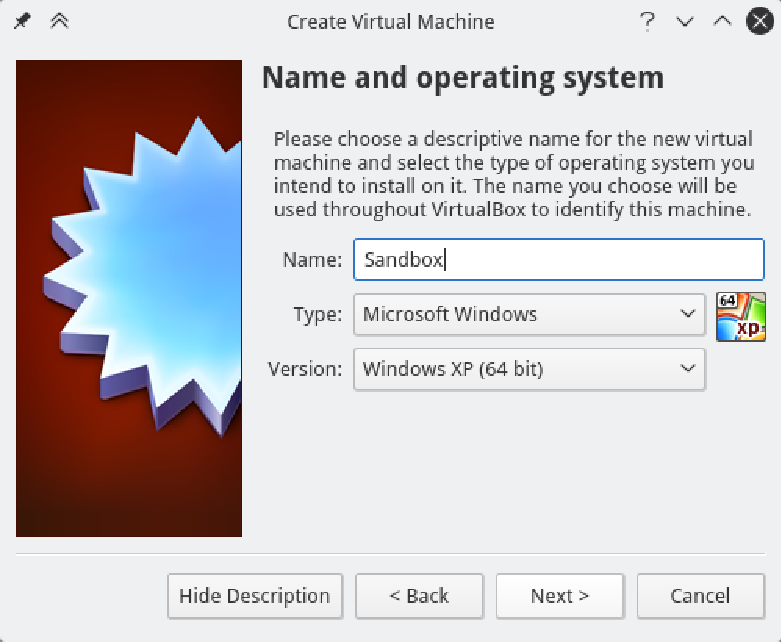
\includegraphics[width=.9\textwidth ,height=.65\textwidth]{Pic/VBox1}
    \caption{ نمایی از ویرچوال باکس}
    \label{VBOX1}
\end{figure}

در مرحله بعدی و در پنجره جدید می‌توانید در نوار لغزان که مشاهده می‌شود، مقدار استفاده از حافظه جانبی را مشخص کنید، در این مورد ما این گزینه را بر روی ۱۰۲۴ مگابایت قرار می‌دهیم که برای اکثر مواقع و در کاربردهای مختلف گزینه خوبی به شمار می‌آید. مراحل باقی مانده مراحل مانند ایجاد دیسک سخت‌افزاری و … را نیز ممکن است، سابقا دیده و استفاده کرده باشید. با این حال در هنگامی که می خواهید نوع دیسک سخت مجازی را انتخاب کنید به جای استفاده از گزینه دینامیک «Dynamic» از گزینه فیکس شده «Fixed»، استفاده کنید.
\begin{figure}
    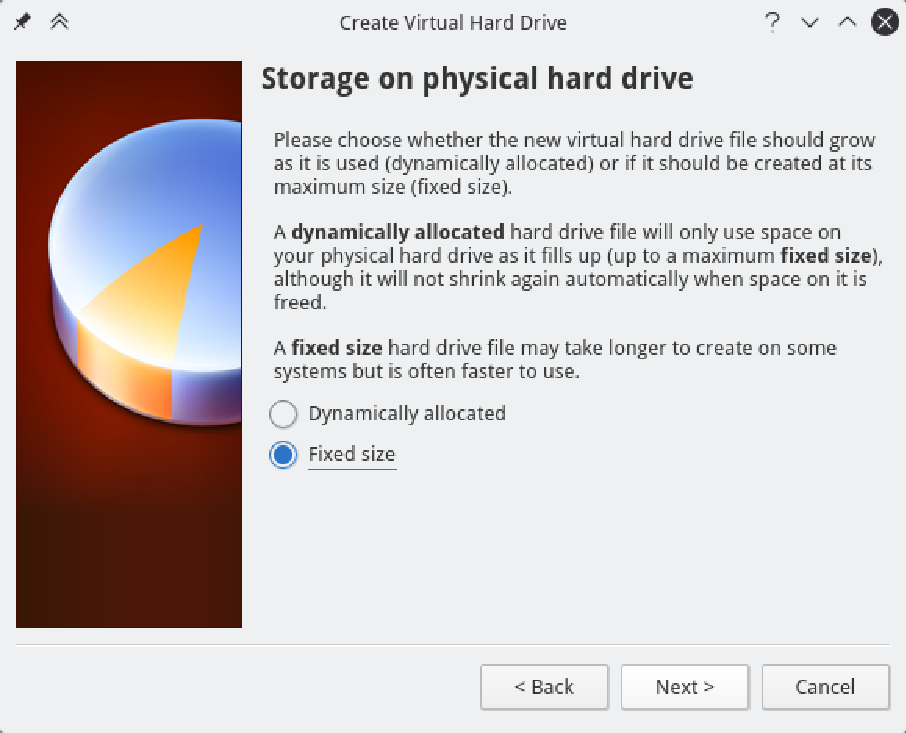
\includegraphics[width=.9\textwidth ,height=.65\textwidth]{Pic/VBox2}
    \caption{ نمایی از ویرچوال باکس}
    \label{VBOX2}
\end{figure}

گزینه پویا و دینامیک باعث می‌شود تا فضای کمتری از دیسک سخت شما اشغال شود و مادامی که از آن استفاده شده است، فضایی را در دیسک سخت اشعال کند، امّا گزینه فیکس شده از همان ابتدا مقدار تعیین شده را از حافظه جدا کرده و به دیسک سخت مجازی نسبت می‌دهد. با وجود صرفه‌جویی در استفاده از فضای دیسک توسط گزینه پویا، با این حال گزینه فیکس شده و ثابت سرعت و کارایی بالاتری را ارائه می‌کند. بنابراین به دلیل ارزانی فضای دیسک و فضای کم مورد نیاز برای نصب توزیع اوبونتو که در این مثال ما از ۸ گیگابایت فضا برای ذخیره اطلاعات نیاز داریم،  این فضا را به صورت یک دیسک سخت مجازی فیکس شده ایجاد می‌کنیم. در این مثال و حتی کاربردهای پیشرفته‌تر به فضای بالاتری نیاز نخواهد بود با این حال اگر داده‌های زیادی را در سندباکس مورد استفاده قرار می‌دهید بهتر است آن را بر روی گزینه‌های بالاتری قرار دهید. در هر صورت فضای ۸ گیگابایت در اکثر مواقع کافی به نظر می‌رسد.

بعد از ایجاد ماشین مجازی حال نوبت به تنظیم آن رسیده است برای اینکه بتوانید آن را تنظیم کنید، باید ابتدا از قسمت سمت راست، ماشین مجازی دلخواه را انتخاب کرده و بر روی گزینه تنظیمات «Settings» کلیک کنید. بعد از کلیک بر روی آن پنجره تنظیمات ماشین مجازی مورد نظر باز خواهد شد. تنظیمات را از بخش پردازنده «CPU» آغاز می‌کنیم. برای این‌کار ابتدا به بخش سیستم «System» رفته و از زیرشاخه پردازنده «CPU»، گزینه 
\lr{«Enable PA/NX»}
 را فعال کنید زیرا که اوبونتو سرور با استفاده از آن می‌تواند پردازشها را سریع‌تر انجام دهد.

بعد از انجام کار قبلی به بخش صدا «Audio» رفته و تیک کنار فعال بودن این بخش را کاملا بردارید، زیرا در این ماشین مجازی ما نیازی به صدا نخواهیم داشت.  در بخش اشتراک پوشه‌ها نیز که با نام 
\lr{«Shared Folders»} 
مشخص است نیز شاخه دلخواه خود را برای اشتراک پوشه  بین میزبان و میهمان مشخص کرده تا بتوانید به آن دسترسی داشته باشید. در هنگام ایجاد پوشه مشترک، دقت کنید که تیک کنار گزینه اتصال خودکار 
\lr{«Auto Mount» }
را بزنید، (یعنی تیک‌دارش کنید) تا در هر بار اجرای ماشین مجازی این پوشه خودکار اشتراک گذاشته شود. سپس وارد بخش ذخیره‌سازی «Storage» شده و با انتخاب نقشک به شکل دیسک نوری، گزینه‌های سمت راست و در کنار لیست تغیر می‌کنند که بعد از تغییر آن گزینه‌ها و کلیک بر نقشک دیسک نوری (دارای فلاشی رو به پایین) واقع در کادر سمت راست و کنار بخش انتخاب دیسک،  در منوی باز شده روی گزینه 
\lr{«choose a virtual cd/dvd image»}
 کلیک کرده سپس در پنجره باز شده برای انتخاب تصویر، تصویر دانلود شده را انتخاب کرده و تایید کنید.

\begin{figure}
    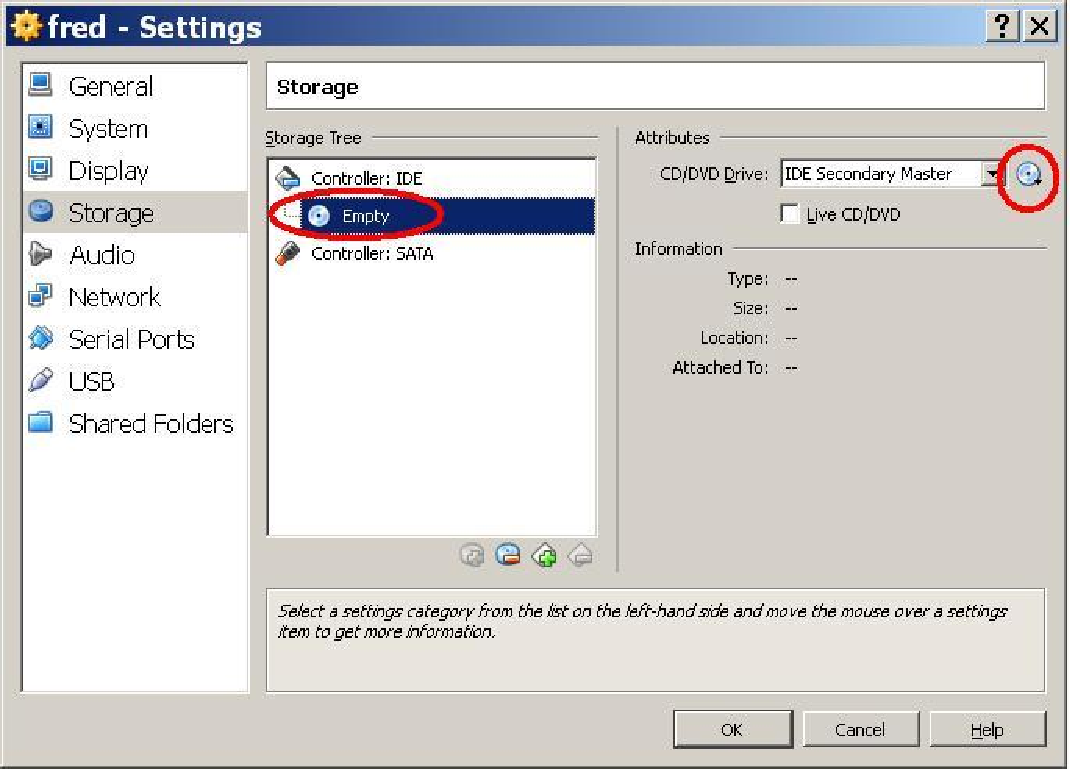
\includegraphics[width=.9\textwidth ,height=.65\textwidth]{Pic/VBox3}
    \caption{ نمایی از ویرچوال باکس}
    \label{VBOX3}
\end{figure}
سپس بعد از اتمام تنظیمات بالا، هنوز کار تمام نشده است، بنابراین پنجره تنظیمات را نبندید و تنظیمات زیر را نیز انجام دهید.

\section{انتقال درگاه 
    \lr{ «Port Forwarding»}}
تنظیمات شبکه به صورت پیش‌فرض در ویرچوال‌باکس بر روی گزینه NAT قرار دارد.  بر اساس تعریف ویکی‌پدیا:

برگردان نشانی شبکه 
\lr{(NAT=Network Address Translation)}
، در شبکه‌بندی رایانه‌ای، روشی است برای فرستادن و دریافت ترافیک شبکه از طریق مسیریاب که با بازنویسی IP منبع و یا مقصد سروکار دارد و گاه نیز با شماره درگاه‌های 
\lr{TCP/UDP }
که بسته‌های IP از آن می‌گذرند، سروکار دارد. می‌توان گفت اگر چند رایانه از راه LAN با هم پیوند دارند و هر یک نشانی IP محلی دارند و می‌خواهند از راه یک رایانه که به شبکه اینترنت پیوند دارد (WAN) و نشانی IP جهانی دارد از اینترنت بهره ببرند، در اینگاه از این روش بهره می‌برند.

\lr{checksums}
 یا اعتبارسنجها
 (
هم
 \lr{IP}
  و هم
 \lr{TCP}
 )
 نیز باید بازنویسی شوند تا تغییر و دگرگونی به کار بسته شود. بیش تر سیستم‌هایی که از 
 \lr{NAT}
  استفاده می‌کنند همین کار را برای توانا کردن چند میزبان بر روی شبکه پوشیده(خصوصی) انجام می‌دهند تا دسترسی به اینترنت از راه یک نشانی IP همگانی (عمومی) ممکن شود. بسیاری از سرپرست‌های شبکه، NAT را روشی آسان می‌دانند و بسیار از آن بهره می‌برند. به هر روی، NAT می‌تواند پیچیدگی‌هایی را در ارتباط و پیوند میان میزبان‌ها (هاست‌ها) ایجاد کند و نیز می‌تواند بر کارکرد اثر بگذارد. (ویکی‌پدیا دانشنامه آزاد)

بنا براین اگر بخواهیم با استفاده از آدرس IP و یا نام دلخواه تنظیم شده در 
\path{«/etc/hosts»}
 دسترسی داشته باشیم باید از قابلیت انتقال درگاه یا پورت فوروارد استفاده کنید. این موضوع باعث می‌شود که به عنوان مثال درگاه شماره ۸۰ را که برای دسترسی به صفحات وب است را از رایانه میهمان به درگاه مثلا ۸۰۸۰ در رایانه میزبان انتقال دهیم. در این صورت هنگامی که در کامپیوتر میزبان از IP کامپیوتر مهمان به همراه درگاه ۸۰  استفاده شود، قادر خواهید بود به صفحه میزبانی شده در  سیستم‌عامل میهمان  که توسط آپاچی آماده شده است، دسترسی داشت. 
بنابراین برای تمامی درگاه‌های مورد نیاز که باید به آنان از طریق میزبان دسترسی داشت، باید درگاه‌ها مورد نظر را از میهمان به درگاه خاصی در میزبان انتقال دهیم. در این مثال ما درگاه ۸۰ را به ۸۰۸۰ و دیگر درگاه‌های مورد نیاز را نیز به این منوال به درگاه بی‌مصرف در میزبان منتقل می‌کنیم.  اگر از درگاه مشابه استفاده کنید، آن درگاه در میزبان برای کاربردهای برنامه‌های میزبان، اشکالاتی را به وجود خواهد آورد. به عنوان نمونه اگر درگاه مای‌اس‌کیو‌ال را با شماره درگاه ۳۳۰۶ به میزبان انتقال دهید آنگاه میزبان قادر نخواهد بود، تا برنامه فوق را اجرا نماید.
\begin{figure}
    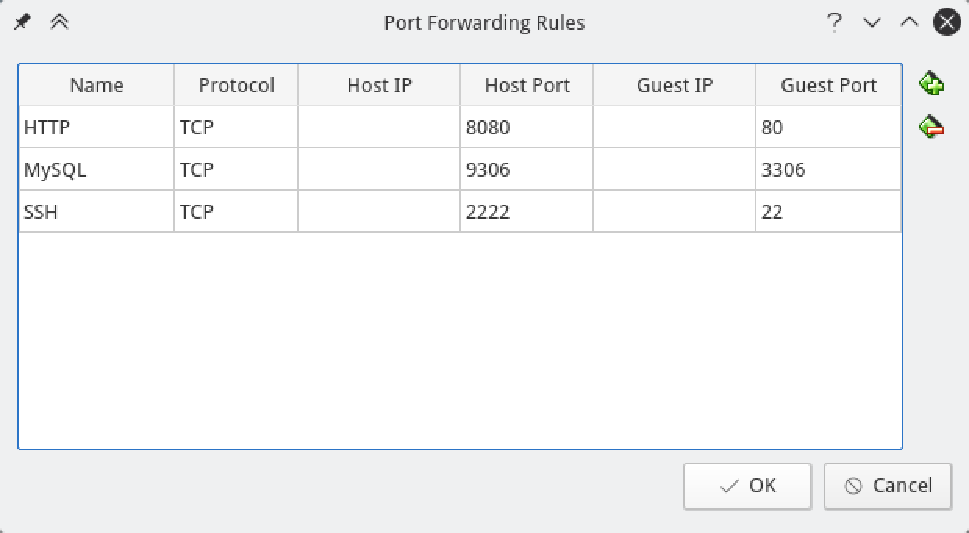
\includegraphics[width=.9\textwidth ,height=.45\textwidth]{Pic/VBox4}
    \caption{ نمایی از ویرچوال باکس}
    \label{VBOX4}
\end{figure}
برای دسترسی به تنظیمات انتقال درگاه در ویرچوال‌باکس وارد تنظیمات شوید، در قسمت شبکه «Network» و با کلیک بر روی گزینه پیشرفته «Advanced» کادر جدید مشاهده خواهد شد،  با کلیک بر روی گزینه انتقال درگاه پنجره محاوره‌ای جدید باز خواهد شد. سپس موارد موجود در تصویر بالا را در آن وارد کنید. برای این‌کار باید روی گزینه اضافه کردن قانون جدید 
\lr{«Insert new rule»}
 کلید کرده تا سطر جدید در جدل اضافه شود، سپس مانند شکل به پر کردن مقادیر و مقادیر دلخواه دیگر بپردازید.
\section{نصب اوبونتو سرور ۱۴٫۰۴}
ابتدا وارد ماشین مجازی شده و بر روی گزینه اجرا «Run» کلیک کرده تا ماشین مجازی اجرا شود. بعد از اجرا اگر پیغامی نمایش داده شد، این پیغام‌ها را تایید کنید و منتظر اجرای صفحه آغازین اوبونتو در اجرای اول در هنگام راه‌اندازی بمانید. صفحه ای با منوی مشابه تصویر نمایش داده خواهد‌شد که بر روی زبان انگلیسی کلید اینتر را از صفحه‌کلید فشار دهید.
\begin{figure}
    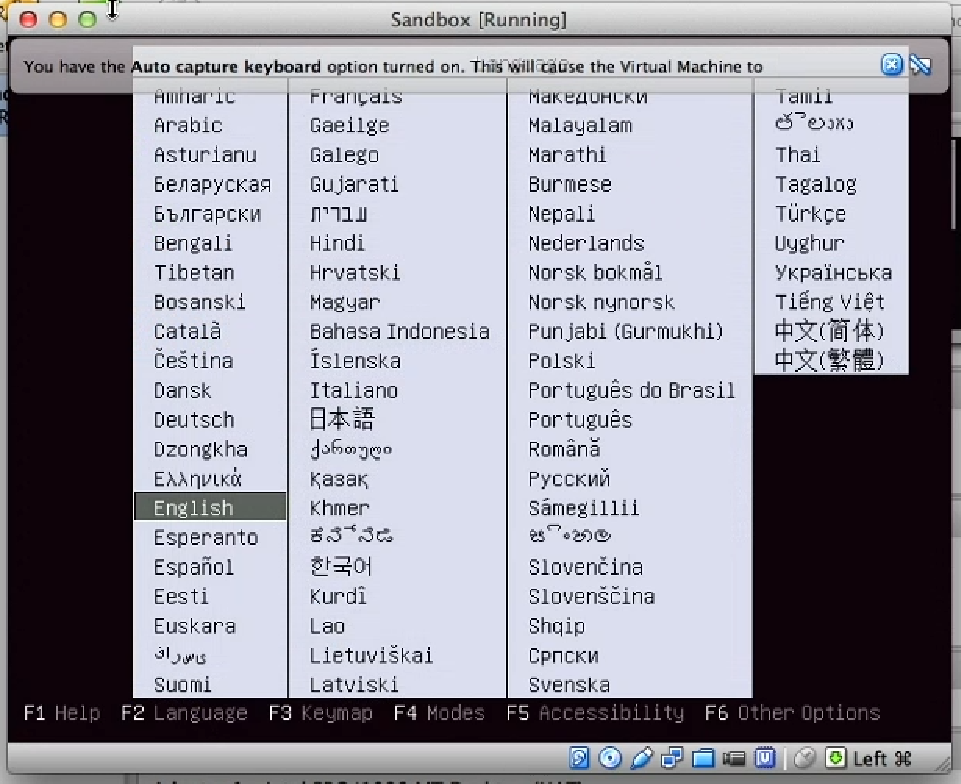
\includegraphics[width=.9\textwidth ,height=.65\textwidth]{Pic/UbuntuServer1}
    \caption{ صفحهٔ بوت اوبونتو سرور}
    \label{UbuntuServer1}
\end{figure}

بعد از آن، باید مد و حالت نصب را به حالت نصبم مینیمال در ویرچوال‌باکس تغییر دهید، در این حالت کلید 
\path{F3}
 را بر روی صفحه‌کلید بفشرید و در منوی ظاهر شده گزینه آخر یعنی نصب مینیمال در ویرچوال‌باکس را انتخاب کنید. بعد از انتخاب حالت نصب بروی گزینه اول یعنی نصب اوبونتو کلیک کنید.
\begin{figure}
    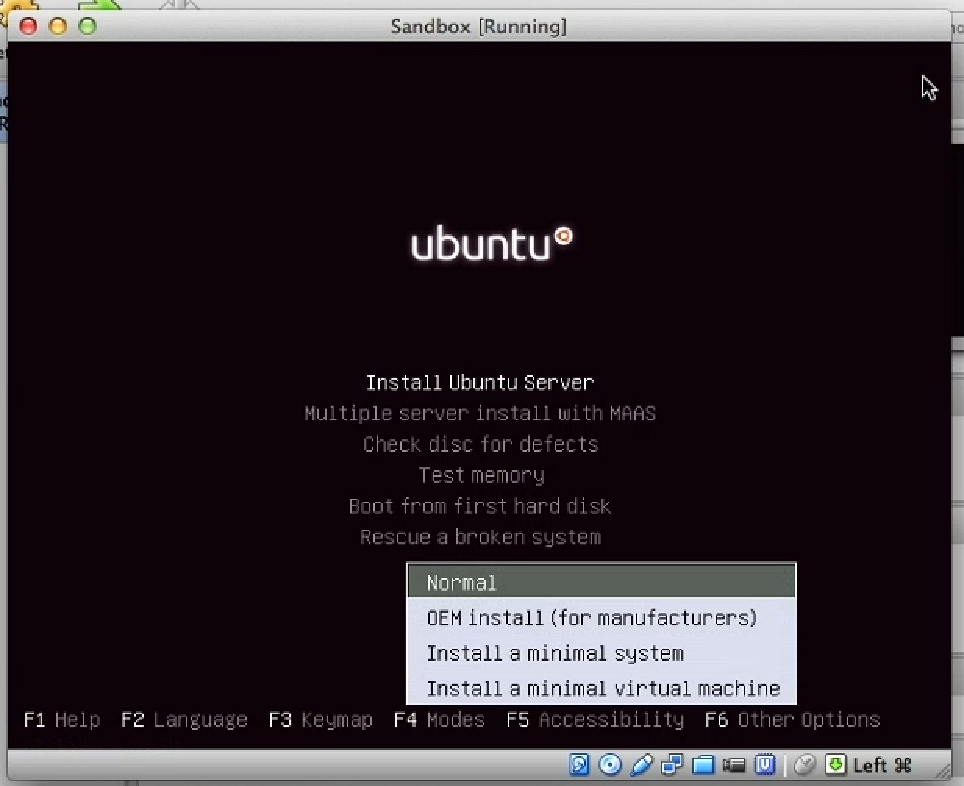
\includegraphics[width=.9\textwidth ,height=.65\textwidth]{Pic/UbuntuServer2}
    \caption{ نصب اوبونتو سرور}
    \label{UbuntuServer2}
\end{figure}

در قسمت بعد به طور مجدد زبان را انتخاب کنید، در قسمت بعدی نیز مکان فعلی خود را انتخاب کنید، که در این مورد ما ایران را انتخاب خواهیم کرد. شما نیز مکان مورد نظر خود را انتخاب کنید. (اگر مورد دیگری است.) از آنجایی که کشور ایران در لیست ابتدایی حضور ندارد، از قسمت گزینه دیگر «Other»  می‌توانید از لیست موجود در این بخش قاره آسیا «Asia» و سپس کشور ایران را انتخاب کنید.  همچنین می‌توانید از دیگر قاره‌ها یا لیست اول، هر کشوری که در آن زندگی می‌کنید را انتخاب کنید. بعد از آن دیسک نوری و سیستم شما بررسی خواهد شد. .

در ادامه فرآیند نصب چند نکته مهم را رعایت کنید، ابتدا پیشنهاد می‌کنم که بهتر است نام سیستم را 
\url{ sandbox.dev}
 قرار دهید و در هنگام موارد مورد نیاز برای نصب همانند تصویر گزینه‌های نصب  \lr{}LAMP و نصب \lr{}SSH را حتما تیک‌دار کنید. برای این‌کار باید از کلید فاصله روی صفحه‌کلید استفاده کنید. بعد از آن در مرحله نوشتن نام کاربری و گذرواژه  باید نام کاربری را مشخص کرده و در کادر وارد کنید , یعنی یک نام کاربری جدید باید بسازید. بعد از انجام امور فوق، بقیه موارد را به دلخواه خود انتخاب کنید.
\\
\begin{figure}
    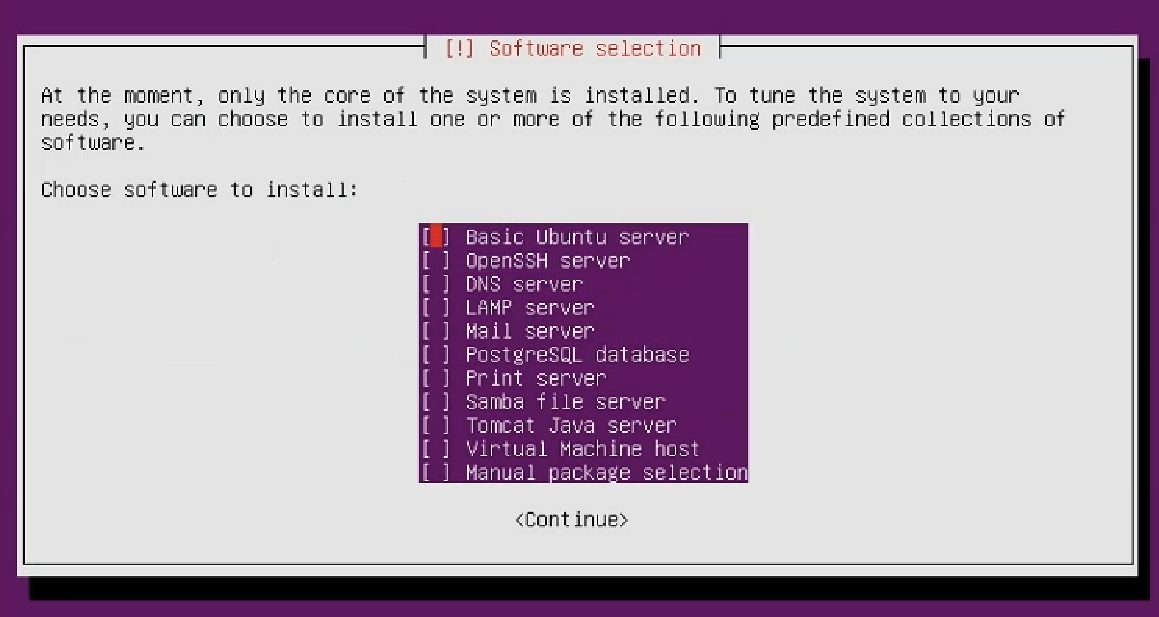
\includegraphics[width=.9\textwidth ,height=.45\textwidth]{Pic/UbuntuServer3}
    \caption{ انتخاب بسته های نرم افزاری برای نصب}
    \label{UbuntuServer3}
\end{figure}

برای پارتیشن‌بندی فضای دیسک بهتر است این‌کار را با استفاده از گزینه اول یعنی خودکار «اتوماتیک» انجام دهید، زیرا که اطلاعات خاصی در ماشین مجازی جود ندارد که نگران پاک شدنشان باشید. این گزینه به پارتیشن‌بندی و تنظیمات ابتدایی خواهد پرداخت. یک فضای Swap در نظر خواهد گرفت به همراه یک پارتیشن برای ریشه و کاربر خانگی که گزینه‌های استانداردی در گنو/لینوکس به شمار می‌آیند.
\begin{figure}
    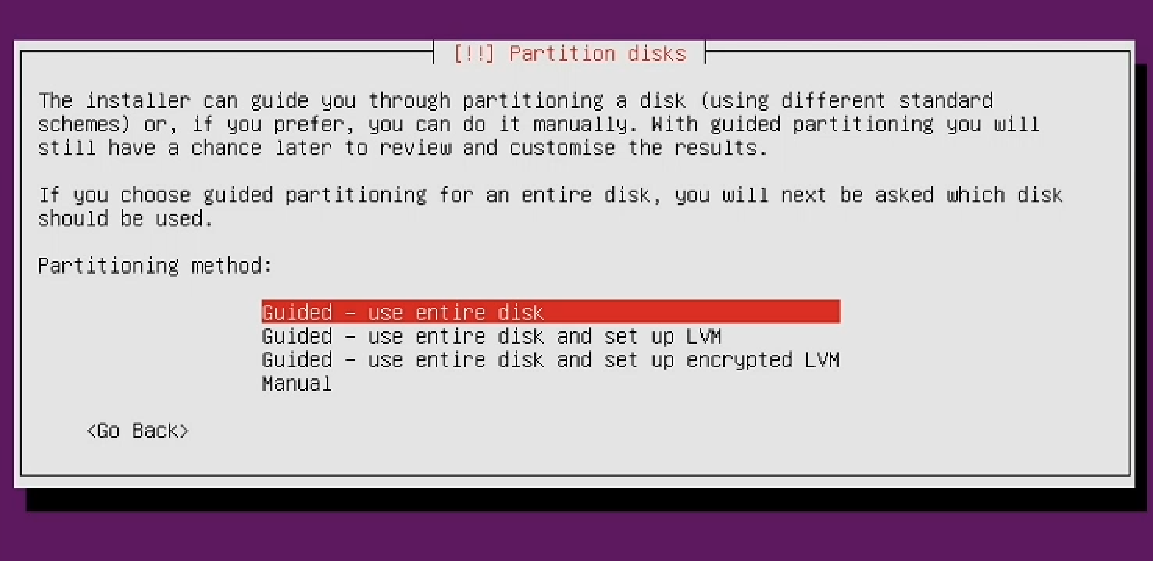
\includegraphics[width=.9\textwidth ,height=.45\textwidth]{Pic/UbuntuServer4}
    \caption{ انتخاب بسته های نرم افزاری برای نصب}
    \label{UbuntuServer4}
\end{figure}

\section{چکیدهٔ فصل}

در این فصل به معرفی گنو/لینوکس و آشنایی و بیان مفاهیمی درباره کارساز وب و سیستم عامل گنو/لینوکس و دیگر موارد پرداختیم که اگر از این موارد اطلاع نداشتید، با آنان آشنا شوید. همچنین در پایان به نحوه تنظیم ویرچوال‌باکس و نصب اوبونتو پرداختیم. در قسمت بعدی این مقالات به تنطیم اوبونتو و سیستم میزان برای دسترسی به مهمان به صورت  \lr{}SSH خواهیم پرداخت. همچنین به نحوه نصب و اجرای چند نرم افزار مورد نیاز برای استفاده در سرور نیز خواهیم پرداخت در آخر اگر مطلب طولانی نشد، نصب چندین ابزار و فریم‌ورک خوب برای پی‌اچ‌پی را  نیز در مطلب  فصل بعد و یا شاید قسمت سوم، معرفی خواهم کرد.

